% first example chapter
% @author Jan Robert Rösler 
%
\chapter{Entwurf}

\note{Hier wird alles erläutert, was ich technisch gemacht habe, siehe Auflistung}


Kenn-Daten von DroNet (Berehcnungszeit, Parameter Layer)


Adaption auf das Carolo Cup Fahrzeug

Performance des Netzes in besimmten Metriken ist nicht intzeressant, da es um die Adaption auf Carolo Teststrecke geht.

Fahren auf der Strecke 

\note{Hervorhaben, welche Teile des DroNet Codes ich weiterverwede. Hard Mining, Auswertungsfunktionen, Architektur}

Änderungen an der Architekrtur des Netzes
Lernarchitekrur (Pipepline)
Steuerungsarchitektur
Bilder mit Steuerdaten (Verarbeitungspipeline) UND VERDOPPELUNG DER DATEN
Fahrzeug (Kamera, Rechner etc.)
Strecke 
Training 
Performance (Rechenzeit) bei prediction auf dem Fahrzeug
Kommunikation zwischen C und pYthon

\note{BILD der STrecke}

\section{Carolo-Cup}
aufgabenstellung beim carolocp
haus eigene strecke etc

\section{Die Strecke}

\section{Das Fahrzeug}
Das Fahrzeug, was von einem Carolo-Cup Team der HAW aufgebaut wurde, wird hier vorgestellt.


\begin{figure}
	\centering
	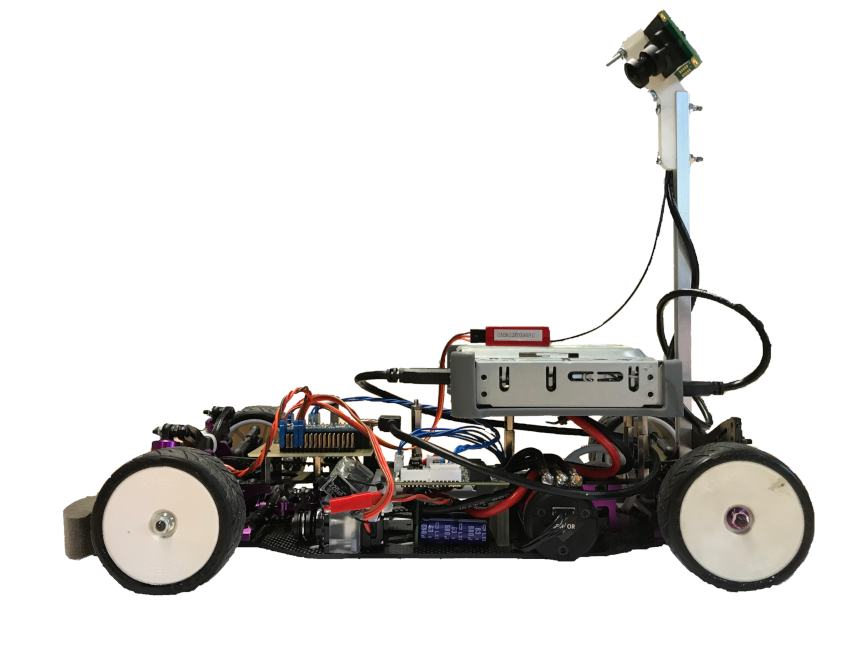
\includegraphics[scale=0.3]{figures/Fahrzeug.png}
	\caption{Das Carolo-Cup Fahrzeug}
	\label{img:Carolo-Fahrzeug}
\end{figure}




Kurzer Blick auf  Self driving car steering angle4 prediction und berkeley (large scale video sets) (vielleicht auchSPÄTER)

